\documentclass[12pt]{article}
\usepackage[pdftex]{graphicx}
\newcommand{\kg}{\mathrm{kg}}
\newcommand{\m}{\mathrm{m}}
\newcommand{\cm}{\mathrm{cm}}
\newcommand{\mm}{\mathrm{mm}}
\newcommand{\km}{\mathrm{km}}
\newcommand{\mi}{\mathrm{mi}}
\newcommand{\s}{\mathrm{s}}
\newcommand{\ms}{\mathrm{ms}}
\newcommand{\h}{\mathrm{h}}
\newcommand{\N}{\mathrm{N}}
\newcommand{\W}{\mathrm{W}}
\newcommand{\hp}{\mathrm{hp}}
\newcommand{\rad}{\mathrm{rad}}
\newcounter{problem}
\stepcounter{problem}
\newcounter{answer}[problem]
\newenvironment{problem}{\noindent\begin{minipage}{\textwidth}\sloppy\sloppypar\raggedright\textbf{\theproblem.}\refstepcounter{problem}\stepcounter{answer}---}{\end{minipage}\vspace{2ex}}
\newcommand{\source}[1]{[{#1}]}
\newenvironment{answers}{\\}{}
\newcommand{\answer}[1]{\textbf{\Alph{answer}:}\refstepcounter{answer}~\mbox{#1\hspace{3ex}}}
\begin{document}

\section*{NYU General Physics 1---Term Exam 3}

\begin{problem}
  \source{from lecture 2011-11-08} If you stretched a guitar string by
  a distance $\Delta L$, how much work did you do?  In these
  equations, $E$ is the elastic modulus, $A$ is the cross-sectional
  area of the string, $L$ is the length of the string, and $M$ is the
  mass of the string.
  \begin{answers}
    \answer{$\displaystyle\frac{1}{2}\,\sqrt{\frac{E\,A}{M\,L}}\,(\Delta L)^2$}
    \answer{$\displaystyle\frac{1}{2}\,\sqrt{\frac{E\,A}{L}}\,(\Delta L)^2$}
    \answer{$\displaystyle\frac{1}{2}\,\frac{E\,A}{M\,L}\,(\Delta L)^2$}
    \answer{$\displaystyle\frac{1}{2}\,\frac{E\,A}{L}\,(\Delta L)^2$}
    \answer{none of these}
  \end{answers}
\end{problem}

\begin{problem}
  \source{from lecture 2011-11-08} If you want to lower the
  fundamental frequency of a piano string of fixed length, you can
  change the tension or the mass.  Which gives the options that lower
  the fundamental frequency?
  \begin{answers}
    \answer{lower the tension or lower the mass}
    \answer{raise the tension or lower the mass}
    \answer{lower the tension or raise the mass}
    \answer{raise the tension or raise the mass}
  \end{answers}
\end{problem}

\begin{problem}
  \source{from lecture 2011-11-10} The length $\ell$ of a pendulum (a
  mass $M$ on the end of a light string of length $\ell$ that ticks
  off seconds (that is, has a two-second period) is about
  \begin{answers}
    \answer{$0.1\,\m$}
    \answer{$1\,\m$}
    \answer{$10\,\m$}
    \answer{$100\,\m$}
    \answer{depends on the mass $M$}
  \end{answers}
\end{problem}

\begin{problem}
  \source{from lecture 2011-11-10} The sine of the very small angle
  $0.01$\,radians is
  \begin{answers}
    \answer{much less than 0.01}
    \answer{very slightly less than 0.01}
    \answer{exactly 0.01}
    \answer{very slightly more than 0.01}
    \answer{much more than 0.01}
  \end{answers}
\end{problem}

\begin{problem}
  \source{from lecture 2011-11-15} A wave has wavelength $\lambda$,
  frequency $f$, and wave speed $v$.  These are related by
  \begin{answers}
    \answer{$\displaystyle v = \frac{1}{\lambda\,f}$}
    \answer{$\displaystyle v = \frac{\lambda}{f}$}
    \answer{$\displaystyle v = \frac{f}{\lambda}$}
    \answer{$\displaystyle v = \lambda\,f$}
    \answer{none of these}
  \end{answers}
\end{problem}

\begin{problem}
  \source{from lecture 2011-11-17} The figure shows a standing wave
  ringing on a string at various different times as it is ringing.  At
  the time marked Q, in what form is the
  energy?\\ 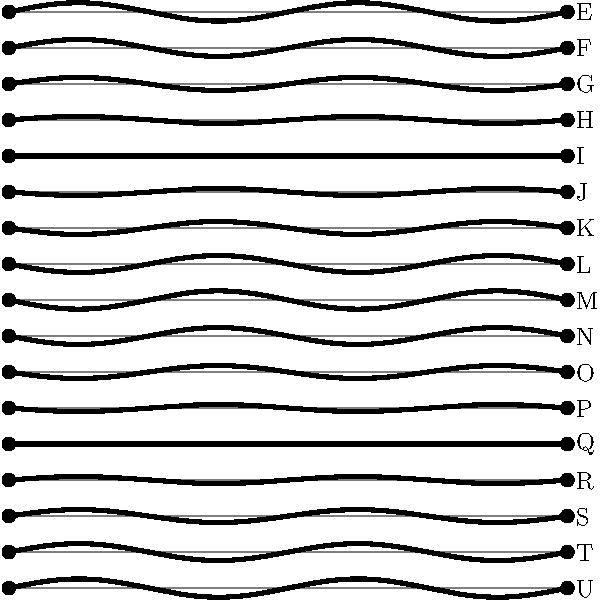
\includegraphics{../py/standing_wave.pdf}
  \begin{answers}
    \answer{potential}
    \answer{kinetic}
    \answer{heat}
    \answer{there is no energy; it is in equilibrium}
    \answer{none of these}
  \end{answers}
\end{problem}

\begin{problem}
  \source{from lecture 2011-11-22} Consider two points in a glass of
  water separated by a vertical distance $\Delta h$.  What is the
  pressure difference $\Delta P$ between those two points?  In these
  equations, $\rho$ is the density of water and $g$ is the
  acceleration due to gravity.
  \begin{answers}
    \answer{$\displaystyle \Delta P = \frac{1}{\rho\,g}\,\Delta h$}
    \answer{$\displaystyle \Delta P = \frac{\rho}{g}\,\Delta h$}
    \answer{$\displaystyle \Delta P = \frac{g}{\rho}\,\Delta h$}
    \answer{$\displaystyle \Delta P = {\rho\,g}\,\Delta h$}
    \answer{it depends on the shape of the glass}
  \end{answers}
\end{problem}

\begin{problem}
  \source{from lecture 2011-11-29} A helium balloon is floating in an
  accelerating bus.  Think of the bus as being a closed tank of air.
  What is the direction of the buoyant force on the balloon?
  \begin{answers}
    \answer{in the direction of decreasing pressure}
    \answer{in the direction of increasing pressure}
    \answer{in the down direction}
    \answer{in the up direction}
    \answer{none of these}
  \end{answers}
\end{problem}

\begin{problem}
  \source{from lecture 2011-12-01} Fluid is flowing through a pipe
  that has a large cross-sectional area at the input end, and a small
  cross-sectional area at the output end.  The fluid velocity
  increases from input to output because
  \begin{answers}
    \answer{the pressure is higher at the output end}
    \answer{the volume per unit time varies along the pipe}
    \answer{all the fluid that enters the pipe must leave}
    \answer{none of these is true}
  \end{answers}
\end{problem}

\begin{problem}
  \source{from lecture 2011-12-06} Water flows out of a small hole in
  the vertical wall of a large water tank.  If water surface is a
  height $h$ above the hole, the velocity $v$ of the water shooting
  out of the hole is roughly
  \begin{answers}
    \answer{$\displaystyle v = \sqrt{\frac{1}{g\,h}}$}
    \answer{$\displaystyle v = \sqrt{\frac{g}{h}}$}
    \answer{$\displaystyle v = \sqrt{\frac{h}{g}}$}
    \answer{$\displaystyle v = \sqrt{{g\,h}}$}
    \answer{none of these}
  \end{answers}
\end{problem}

\begin{problem}
  \source{from problem set 9, problem 1} Which is the higher
  frequency?  The frequency of oscillation of a femur bone if you hit
  it so it ``rings'' like a bell because of its own elasticity and
  mass, or the frequency if you swing it like a pendulum in gravity?
  \begin{answers}
    \answer{rings at higher frequency}
    \answer{rings and swings at similar frequencies}
    \answer{swings at higher frequency}
    \answer{there is no way to answer this question}
  \end{answers}
\end{problem}

\begin{problem}
  \source{from problem set 9, problem 2} A mass is oscillating on an
  ideal spring.  Imagine a plot of the total energy $E$ in the oscillator
  as a function of time $t$.
  \begin{answers}
    \answer{The graph oscillates at the frequency of the oscillator.}
    \answer{The graph oscillates at twice the frequency of the oscillator.}
    \answer{The graph is constant with time.}
    \answer{none of these}
  \end{answers}
\end{problem}

\begin{problem}
  \source{from problem set 9, problem 3} What is the second derivative
  with respect to time $t$ of
  $$A\,\cos(\omega\,t + \phi)\quad ,$$
  where $A$, $\omega$, and $\phi$ are all constants?
  \begin{answers}
    \answer{$-\omega^2\,A\,\cos(\omega\,t + \phi)$}
    \answer{$-\omega\,A\,\sin(\omega\,t + \phi)$}
    \answer{$\omega^2\,A\,\cos(\omega\,t + \phi)$}
    \answer{$\omega\,A\,\sin(\omega\,t + \phi)$}
    \answer{none of these}
  \end{answers}
\end{problem}

\begin{problem}
  \source{from problem set 10, problem 1} If you kept the room at
  constant temperature and pressure, but changed the air to helium
  gas, the mass density of the air would drop by a factor of about 4.
  The speed of sound in the room would
  \begin{answers}
    \answer{increase by factor of about 4}
    \answer{increase by factor of about 2}
    \answer{stay about the same}
    \answer{decrease by factor of about 2}
    \answer{decrease by factor of about 4}
  \end{answers}
\end{problem}

\begin{problem}
  \source{from problem set 10, problem 1} An organ pipe that plays
  middle $C$ is about how long?
  \begin{answers}
    \answer{100 feet}
    \answer{10 feet}
    \answer{1 foot}
    \answer{1 inch}
    \answer{none of these}
  \end{answers}
\end{problem}

\begin{problem}
  \source{from problem set 10, problem 2} A transverse wave obeys the
  description
  $$y = A\,\cos\left(\frac{2\pi\,x}{\lambda}-\frac{2\pi\,t}{T}\right)\quad ,$$
  where $A$ is a constant, $\lambda$ is the wavelength, and $T$ is the
  period.  Which way is the wave moving?
  \begin{answers}
    \answer{negative $x$ direction}
    \answer{positive $x$ direction}
    \answer{negative $y$ direction}
    \answer{positive $y$ direction}
    \answer{none of these}
  \end{answers}
\end{problem}

\begin{problem}
  \source{from problem set 10, problem 3} You hit a bell once with a
  hammer.  It rings but the sound it makes decays---it gets softer and
  softer over time.  Why does this happen?
  \begin{answers}
    \answer{Energy is not conserved.}
    \answer{It radiates energy to it's surroundings (including your ears).}
    \answer{The energy has to return to the hammer.}
    \answer{Energy is changing from kinetic to potential and back.}
    \answer{none of these}
  \end{answers}
\end{problem}

\begin{problem}
  \source{from problem set 11, problem 1} A pressure difference of
  $50\,\mm$ of mercury corresponds to roughly how many atmospheres?
  \begin{answers}
    \answer{0.07\,atm}
    \answer{0.7\,atm}
    \answer{1\,atm}
    \answer{10\,atm}
    \answer{none of these}
  \end{answers}
\end{problem}

\begin{problem}
  \source{from problem set 11, problem 1} Airplanes fly at an altitude
  of about $10\,\km$; what is true about this?
  \begin{answers}
    \answer{The density of air is lower at this altitude.}
    \answer{It is much hotter at this altitude.}
    \answer{The speed of sound is much higher at this altitude.}
    \answer{There is no atmosphere at all at this altitude.}
    \answer{none of these}
  \end{answers}
\end{problem}

\begin{problem}
  \source{from problem set 11, problem 2} For a submerged ice cube in
  cold water, the buoyant force is greater than the gravitational
  force.  By what factor is it greater?
  \begin{answers}
    \answer{Infinitely}
    \answer{A factor of 10.8}
    \answer{A factor of 1.92}
    \answer{A factor of 1.08}
    \answer{nothing near any of these}
  \end{answers}
\end{problem}

\begin{problem}
  \source{from problem set 11, problem 3} Consider two cylindrical
  tubes, each carrying 5 liters per minute of blood.  If the wide tube
  has cylindrical radius $1\,\cm$ and the narrow tube has cylindrical
  radius $0.5\,\cm$, what is the ratio of velocities (wide tube
  velocity over narrow tube velocity)?
  \begin{answers}
    \answer{1}
    \answer{0.707}
    \answer{0.5}
    \answer{0.25}
    \answer{none of these}
  \end{answers}
\end{problem}

\begin{problem}
  \source{from \textit{Collisions in One Dimension} lab} A glider of
  mass $m_1$ initially moves at speed $v_1$ in the positive $x$
  direction.  It collides elastically with a second glider of mass
  $m_2$ initially at rest.  Under what condition will the first glider
  continue to move in the positive $x$ direction after the elastic
  collision?
  \begin{answers}
    \answer{$m_1 < m_2$}
    \answer{$m_1 > m_2$}
    \answer{$m_1\,v_1 > m_2$}
    \answer{$m_1\,v_1 < m_2$}
    \answer{none of these}
  \end{answers}
\end{problem}

\begin{problem}
  \source{from \textit{Ballistic Pendulum} lab} A ball of mass $m$
  hits a pendulum bob of mass $M$ and sticks.  Immediately after it
  sticks to the bob, the kinetic energy of the bob+ball system is
  \begin{answers}
    \answer{greater than the initial kinetic energy of the ball}
    \answer{the same as the initial kinetic energy of the ball}
    \answer{less than the initial kinetic energy of the ball}
    \answer{there is not enough information to tell}
  \end{answers}
\end{problem}

\begin{problem}
  \source{from \textit{Work--Energy} lab} You do work $W$ on a mass
  $m$ and all the work goes into increasing the kinetic energy of the
  mass.  If the mass starts off at speed $v_i$ and gains speed $\Delta
  v$ (to end up at speed $v_f = v_i + \Delta v$), then
  \begin{answers}
    \answer{$\displaystyle W = \frac{1}{2}\,m\,(\Delta v)^2$}
    \answer{$\displaystyle W = \frac{1}{2}\,m\,v_i^2$}
    \answer{$\displaystyle W = \frac{1}{2}\,m\,v_i\,(\Delta v)$}
    \answer{$\displaystyle W = \frac{1}{2}\,m\,(v_i + \Delta v)^2$}
    \answer{$\displaystyle W = \frac{1}{2}\,m\,\left[(v_i + \Delta v)^2 - v_i^2\right]$}
  \end{answers}
\end{problem}

\begin{problem}
  \source{from \textit{Oscillations of a String} lab} At fixed string
  tension, as the wavelength of the standing waves gets shorter, the
  frequency of the waves
  \begin{answers}
    \answer{gets smaller}
    \answer{stays the same}
    \answer{gets higher}
    \answer{there is not enough information to tell}
  \end{answers}
\end{problem}

\end{document}
